%%
%% This is file `sample-sigconf.tex',
%% generated with the docstrip utility.
%%
%% The original source files were:
%%
%% samples.dtx  (with options: `sigconf')
%% 
%% IMPORTANT NOTICE:
%% 
%% For the copyright see the source file.
%% 
%% Any modified versions of this file must be renamed
%% with new filenames distinct from sample-sigconf.tex.
%% 
%% For distribution of the original source see the terms
%% for copying and modification in the file samples.dtx.
%% 
%% This generated file may be distributed as long as the
%% original source files, as listed above, are part of the
%% same distribution. (The sources need not necessarily be
%% in the same archive or directory.)
%%
%% The first command in your LaTeX source must be the \documentclass command.
\documentclass[sigconf]{acmart}
\settopmatter{printacmref=false}
% \pagestyle{plain}
\renewcommand\footnotetextcopyrightpermission[1]{}
\usepackage{graphics}
%%%% As of March 2017, [siggraph] is no longer used. Please use sigconf (above) for SIGGRAPH conferences.

%%%% Proceedings format for SIGPLAN conferences 
% \documentclass[sigplan, anonymous, review]{acmart}

%%%% Proceedings format for SIGCHI conferences
% \documentclass[sigchi, review]{acmart}

%%%% To use the SIGCHI extended abstract template, please visit
% https://www.overleaf.com/read/zzzfqvkmrfzn

%%
%% \BibTeX command to typeset BibTeX logo in the docs
\AtBeginDocument{%
  \providecommand\BibTeX{{%
    \normalfont B\kern-0.5em{\scshape i\kern-0.25em b}\kern-0.8em\TeX}}}

%% Rights management information.  This information is sent to you
%% when you complete the rights form.  These commands have SAMPLE
%% values in them; it is your responsibility as an author to replace
%% the commands and values with those provided to you when you
%% complete the rights form.
\setcopyright{acmcopyright}
\copyrightyear{2018}
\acmYear{2018}
\acmDOI{10.1145/1122445.1122456}

%% These commands are for a PROCEEDINGS abstract or paper.
% \acmConference[Woodstock '18]{Woodstock '18: ACM Symposium on Neural
%   Gaze Detection}{June 03--05, 2018}{Woodstock, NY}
% \acmBooktitle{Woodstock '18: ACM Symposium on Neural Gaze Detection,
%   June 03--05, 2018, Woodstock, NY}
% \acmPrice{15.00}
% \acmISBN{978-1-4503-9999-9/18/06}


%%
%% Submission ID.
%% Use this when submitting an article to a sponsored event. You'll
%% receive a unique submission ID from the organizers
%% of the event, and this ID should be used as the parameter to this command.
%%\acmSubmissionID{123-A56-BU3}

%%
%% The majority of ACM publications use numbered citations and
%% references.  The command \citestyle{authoryear} switches to the
%% "author year" style.
%%
%% If you are preparing content for an event
%% sponsored by ACM SIGGRAPH, you must use the "author year" style of
%% citations and references.
%% Uncommenting
%% the next command will enable that style.
%%\citestyle{acmauthoryear}

%%
%% end of the preamble, start of the body of the document source.
\begin{document}

%%
%% The "title" command has an optional parameter,
%% allowing the author to define a "short title" to be used in page headers.
\title{A Study on Kubernetes}

%%
%% The "author" command and its associated commands are used to define
%% the authors and their affiliations.
%% Of note is the shared affiliation of the first two authors, and the
%% "authornote" and "authornotemark" commands
%% used to denote shared contribution to the research.

\author{Udhav Sethi}
\affiliation{\institution{University of Waterloo}}
\email{udhav.sethi@uwaterloo.ca}

\author{Xiyang Feng}
\affiliation{\institution{University of Waterloo}}
\email{x74feng@uwaterloo.ca}

%%
%% By default, the full list of authors will be used in the page
%% headers. Often, this list is too long, and will overlap
%% other information printed in the page headers. This command allows
%% the author to define a more concise list
%% of authors' names for this purpose.
%\renewcommand{\shortauthors}{Trovato and Tobin, et al.}

%%
%% The abstract is a short summary of the work to be presented in the
%% article.
\begin{abstract}
Containerization is taking hold in the datacenter. To leverage the benefits of an isolated environment provided by containers while utilizing resources efficiently, orchestration becomes necessary. Kubernetes is a container orchestration system that allows better tracking, scheduling and operationalizing of containers at scale and eliminates infrastructure complexity. We study and evaluate Kubernetes performance against native application deployment for different workloads. We also conduct a case study on running MongoDB on Kubernetes and discuss the benefits and trade-offs.
\end{abstract}

%%
%% The code below is generated by the tool at http://dl.acm.org/ccs.cfm.
%% Please copy and paste the code instead of the example below.
%%
% \begin{CCSXML}
% <ccs2012>
%  <concept>
%   <concept_id>10010520.10010553.10010562</concept_id>
%   <concept_desc>Computer systems organization~Embedded systems</concept_desc>
%   <concept_significance>500</concept_significance>
%  </concept>
%  <concept>
%   <concept_id>10010520.10010575.10010755</concept_id>
%   <concept_desc>Computer systems organization~Redundancy</concept_desc>
%   <concept_significance>300</concept_significance>
%  </concept>
%  <concept>
%   <concept_id>10010520.10010553.10010554</concept_id>
%   <concept_desc>Computer systems organization~Robotics</concept_desc>
%   <concept_significance>100</concept_significance>
%  </concept>
%  <concept>
%   <concept_id>10003033.10003083.10003095</concept_id>
%   <concept_desc>Networks~Network reliability</concept_desc>
%   <concept_significance>100</concept_significance>
%  </concept>
% </ccs2012>
% \end{CCSXML}

% \ccsdesc[500]{Computer systems organization~Embedded systems}
% \ccsdesc[300]{Computer systems organization~Redundancy}
% \ccsdesc{Computer systems organization~Robotics}
% \ccsdesc[100]{Networks~Network reliability}

%%
%% Keywords. The author(s) should pick words that accurately describe
%% the work being presented. Separate the keywords with commas.
\keywords{Kubernetes, Containers, Distributed Systems}

%% A "teaser" image appears between the author and affiliation
%% information and the body of the document, and typically spans the
%% page.
% \begin{teaserfigure}
%   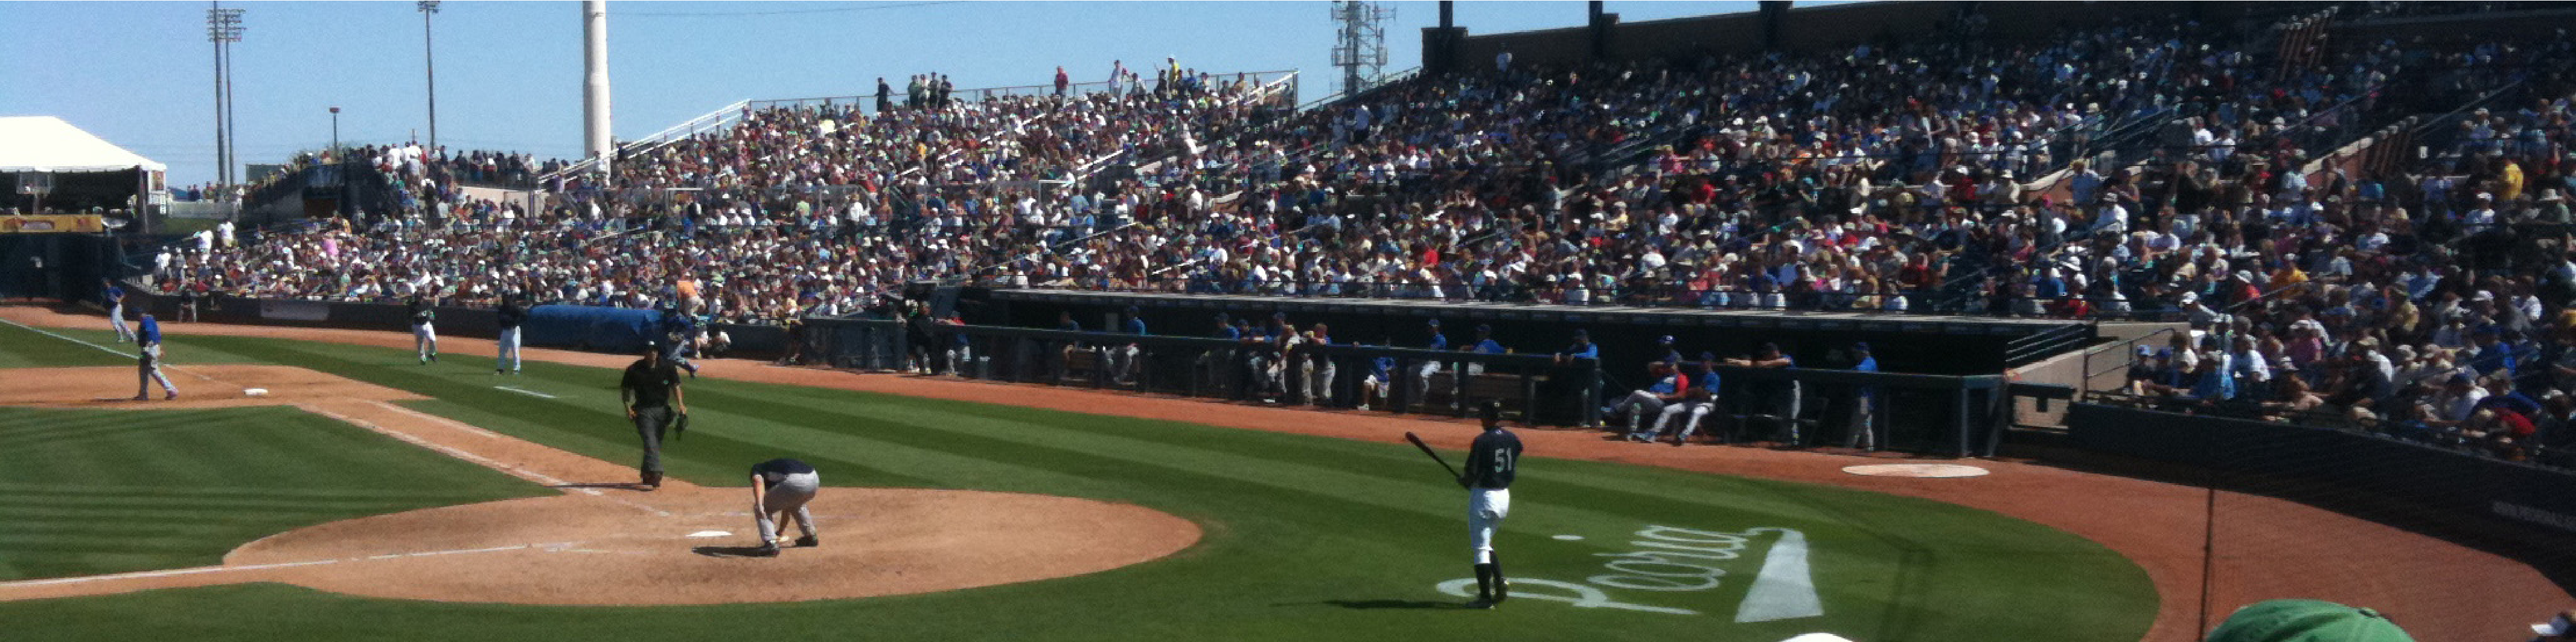
\includegraphics[width=\textwidth]{sampleteaser}
%   \caption{Seattle Mariners at Spring Training, 2010.}
%   \Description{Enjoying the baseball game from the third-base
%   seats. Ichiro Suzuki preparing to bat.}
%   \label{fig:teaser}
% \end{teaserfigure}

%%
%% This command processes the author and affiliation and title
%% information and builds the first part of the formatted document.
\maketitle

\section{Introduction}
In traditional application deployments, applications developed in one computing environment often run into bugs and errors when deployed in another environment. The differences in network topology, storage management, and security policies are some of the variables that lead to issues in the application execution. Containerization attempts to solve this problem by providing an isolated runtime environment to run the application. The application is  bundled together with its dependencies, libraries, binaries, and configuration files into a single package and is run inside a container. Thus, containerization abstracts away the differences in the underlying infrastructure.

Since each container operates independently of others, containers need to be monitored and orchestrated to track all the moving parts and ensure their efficient functioning. Kubernetes is an open-source container-orchestration layer for automating application deployment, scaling, and management.\cite{hightower2017kubernetes} It groups containers that make up an application into logical units for easy management and discovery. Kubernetes enables deployment of a cluster that is highly available, uses resources efficiently, self-heals in case of failures, and scales automatically.

In this paper, we study and evaluate the Kubernetes system. We try to understand its basic functioning, scheduling, and fault-tolerance mechanisms. For evaluation, we first compare the performance of the Kubernetes system in basic tasks, such as ping, CPU intensive and memory intensive workloads against native machine deployments. We then conduct a case study on running the MongoDB application on Kubernetes and investigate the motivation and challenges involved in deployment of such a system. For evaluation, we conduct failover testing on the cluster and also benchmark the performance of the system for the YCSB (Yahoo! Cloud Serving Benchmark) workload.


\section{Kubernetes Architecture}
Kubernetes is built to manage a large number of containers running in a distributed system resiliently. The various components that form the Kubernetes architecture are outlined in Figure 1 and described in the following sections.

\subsection{Kubernetes Clusters}
Kubernetes coordinates a cluster of computers running containerized applications and automates the distribution and scheduling of application containers across a cluster in a more efficient way. A Kubernetes cluster consists of a master and workers. The master coordinates all activities in the cluster, such as scheduling applications, maintaining applications' desired state, scaling applications, and rolling out new updates. A worker machine runs the application. The Kubernetes architecture is outlined in Figure 1.

\subsection{Deployments}
A Deployment instructs Kubernetes how to create application instances onto individual Nodes in the cluster.  If the Node hosting an instance goes down or is deleted, the Deployment controller replaces the instance with an instance on another Node in the cluster. This provides a self-healing mechanism to address machine failure or maintenance.

\subsection{Pods}
A Pod is a Kubernetes abstraction for a “logical host” that represents a group of one or more application containers, and some shared resources (such as storage, IP address, ports) for those containers. Containers in a Pod are always co-located and co-scheduled, and run in a shared context on the same Node. A Pod is an atomic unit on the Kubernetes platform.

\subsection{Nodes}
A Node is a worker machine in Kubernetes and may be either a virtual or physical machine. Every Node has a Kubelet, an agent for managing the pods running on the node and communicating with the Kubernetes master, and a container runtime, responsible for pulling the container image from a registry, unpacking the container, and running the application.

\subsection{Services}
A Service is an abstraction which defines a logical set of Pods and enables loose coupling between them. Services enable external traffic exposure, load balancing and service discovery for those Pods.

\begin{figure}[h]
  \centering
  \def\svgwidth{\columnwidth}
%   \input{kube-arch.pdf_tex}
  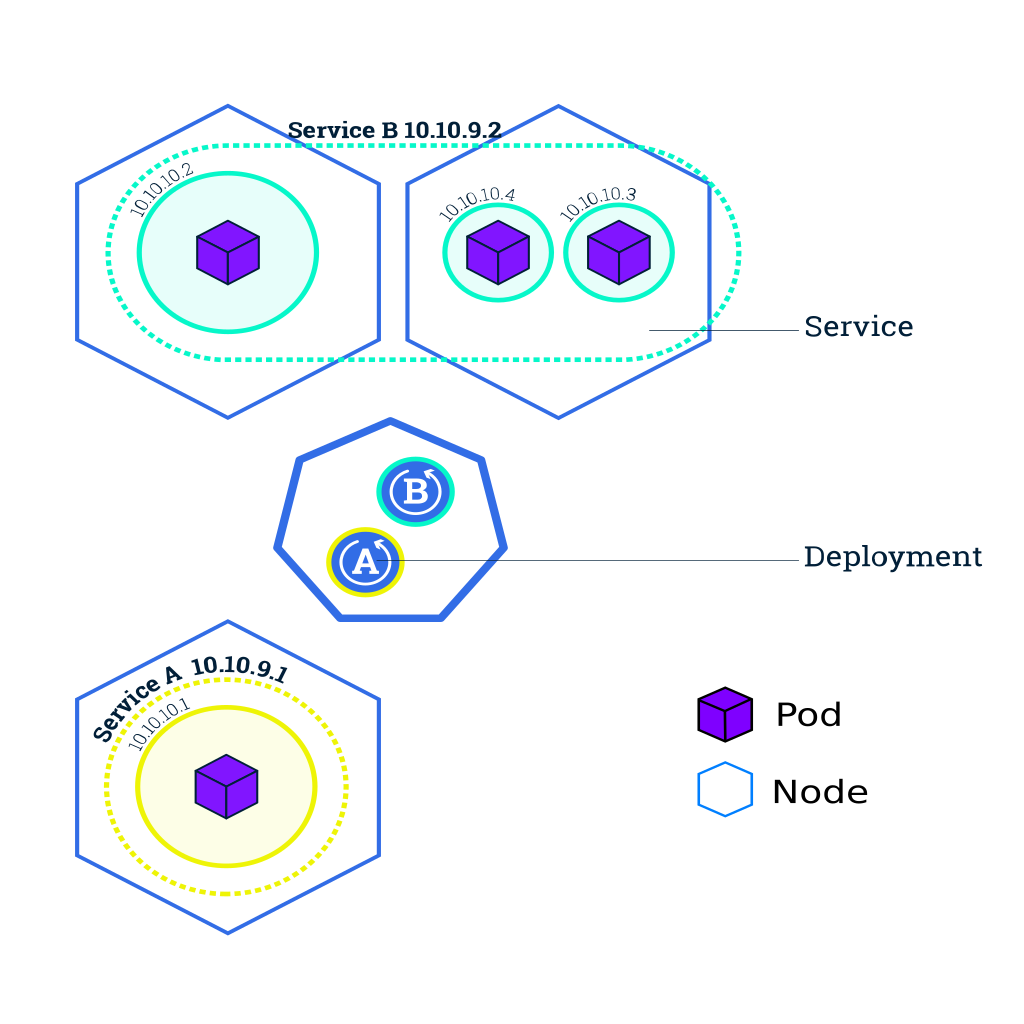
\includegraphics[width=\linewidth]{kube-arch.png}
  \caption{Kubernetes Architecture}
\end{figure}

\subsection{Scaling}
Horizontal Scaling is accomplished by changing the number of replicas in a Deployment, which creates new Pods and schedules them to Nodes with available resources. Kubernetes also supports autoscaling of Pods, where the number of pods are automatically scaled up based on observed CPU utilization or other application-provided metrics.

\subsection{Updates}
Kubernetes provides rolling updates, which allows Deployments to be updated with zero downtime by incrementally updating old Pod instances with new ones. If a Deployment is exposed publicly, the Service will load-balance the traffic only to available Pods during the update.

\section{Networking}

Kubernetes dictates particular requirements on any networking implementation.\cite{KubernetesNetworking}. It is specific about its choices on how Pods are networked. We study these networking models in the sections below.


\subsection{Container-to-Container Networking}
Each pod running on a node is assigned its own network namespace. All the containers within a pod are assigned the same IP address and port space through the namespace of the Pod that encapsulates them. Since they reside in the same namespace, they are able to communicate with each other through localhost.

\subsection{Pod-to-Pod Networking}
Since all the pods have their own network namespace, they communicate with other pods using the IP address assigned to them. The mechanism differs based on if the two pods reside on the same node or different nodes.

\subsubsection{Pods on same Node}

The network namespace assigned to a pod isolates it to its own networking stack. Since all the pods in a node are connected to the root namespace of the node, they go through it to communicate with each other. For this, they use a network bridge that maintains a forwarding table between sources and destinations and connects the namespaces of each of the pods to the root namespace.

\subsubsection{Pods across Nodes}
In Kubernetes, the IP address of a pod is always visible to other pods in the network. The pods residing on different nodes can reach each other through their IP addresses. A pod that wants to communicate with a pod on another node forwards the packet to the network bridge of the root namespace, from where it enters the network. The network forwards the packet to the root namespace of the destination Node, where it is routed through the bridge to the namespace of the destination pod.

\subsection{Pod-to-Service Networking}
Pods are mortal. Pods may be added to or removed from nodes while scaling the application or in case of node failures. A Kubernetes Service solves this problem by tracking the changing pod IP addresses. A service is assigned a virtual IP address which does not change over time. To reach the set of pods associated with a service, the traffic is forwarded to the virtual IP of the service. Kubernetes maintains an internal load balancer that distributes the load among these pods. Thus, in terms of networking, the service acts like a black box that encapsulates all the pods associated with it.

\subsection{Internet-to-Service Networking}
A Kubernetes Service is generally created by specifying a load balancer which is provided by the cloud controller. The IP address of this load balancer is used to direct external traffic to the service. To get traffic from a service out to the Internet, it is forwarded to an Internet gateway which forwards it to the the public Internet.

\section{Scheduling}

The scheduling framework in Kubernetes attempts to schedule a Pod in two phases, the scheduling cycle and the binding cycle. 

Every Pod that is newly created or unscheduled gets added to a Pod queue. In the scheduling cycle, a pod is dequeued from the queue and the scheduler is responsible for finding the optimal Node for that Pod to run on. Since every Pod and every container in the Pod may have different requirements, it is important to first find the nodes that are capable of running the Pod, and then choosing one of them. The scheduler selects a Node for the Pod in 2 steps: filtering, and scoring. These are described in sections 4.1 and 4.2 below.

\subsection{Filtering Step}
The filtering step finds the set of Nodes where it’s feasible to schedule the Pod. The scheduler follows a defined set of filtering policies to find the list of suitable Nodes. Filtering policies are hard constraints and cannot be violated while finding feasible nodes. Some of these policies are listed below:
\begin{itemize}
\item Matching the hostname specified by the Pod.
\item Checking if the Node meets the resource requirements like CPU and Memory specified by the Pod
\item Checking if the ports requested by a Pod are free on the Node.
\item Matching the Volumes requested by the Pod to the mounted volumes on the Node.
\item Fitering out the Nodes reporting storage/memory/PID pressure.
\item Fitering out nodes with completely full filesystem.
\item Marking a node tainted so that no pods can schedule onto it unless a Pod explicitly tolerates the taint.
\end{itemize}

\subsection{Scoring Step}
Once a list of suitable nodes is determined, the scoring step scores the feasible Nodes and picks a Node with the highest score among the feasible ones to run the Pod. Scoring policies are soft constraints and are followed on a best-effort basis. Some of these policies are a part of the Kubernetes scheduler’s default behavior, while others are user-configurable. Some commonly used policies are listed below:
\begin{itemize}
\item Favouring nodes with fewer/more requested resources.
\item Spreading pods among nodes.
\item Prioritizing nodes according to pod affinity/anti-affinity.
\item Balancing out the resource utilization of nodes.
\item Favouring nodes that already have the container images for that Pod cached locally.
\item Co-locating services that communicate frequently.
\item Simply allocating equal weights to all nodes.
\end{itemize}

On having selected an optimal Node for running a Pod, the binding cycle applies that decision to the cluster. A scheduling or binding cycle can be aborted if the Pod is determined to be unschedulable or if there is an internal error. The Pod will be returned to the queue.

\section{Failure Handling}
Kubernetes features a self-healing mechanism so that the system remains highly available. The Replication Controller feature helps Kubernetes achieve high availability through failures. We will talk about the Replication Controller feature and the various failure scenarios in the following sections.

\subsection{Kubernetes Replication Controller}
The Replication Controller feature of Kubernetes is responsible for managing the pod lifecycle through supervision of multiple pods across multiple nodes.\cite{ReplicationControllers} A Replication Controller ensures that a specified number of pod replicas are up and running at any given time. Depending upon the number of pods specified for the application, the Replication Controller adds more pods or terminates extra pods.

The motivation behind replicating application containers is to achieve reliability, scalability, and load-balancing for the application. The goal of Replication Controller is that the services and their clients should remain oblivious to the underlying process of maintaining a fixed number of replicas in the cluster. The Replication Controller makes it easy to scale the number of replicas up or down, either manually or by an auto-scaling control agent, by simply updating the replicas field.


\subsection{Worker Failure}
The kubelet on each worker node posts a node status to the master every fixed interval of time. The frequency is determined by the node status update frequency (default=40s). If the node is unresponsive for a grace period (default=40s), the node is marked as unhealthy. Once the node is marked unhealthy for longer than the pod eviction grace period (default=5m), all the pods on the node are marked for eviction. Thereafter, no traffic is routed to the pods marked for eviction.

If a node crashes, the above mechanism will kick in and the pods scheduled on the failed node will be evicted from the cluster. In such a scenario, the Replication Controller tries to ensure that the desired number of pods matches its label selector and are operational. It adds the required additional pods to the available healthy nodes in the cluster so that the cluster state is restored.

\subsection{Master Failure}
The master is responsible for managing and coordinating the cluster. If the master goes down, the cluster is no longer able to create new resources, reschedule pods among worker nodes, or respond to worker node failures. Since the other services such as DNS, load balancing etc. continue to function, the application  continues to function normally in the absence of failures. The auto-scaling, self-healing nature of the cluster is no longer operational.

\subsection{Network Partition}
In case of a network partition between the master and a worker node, no traffic is able to be sent to or received from the worker node. In such a scenario, a similar mechanism to worker node failure causes the Replication Controller to perceive those pods to be terminated or deleted. The unreachable node is dropped from the cluster and all its pods are rescheduled to other hosts.

\begin{figure*}[ht] 
  \label{simple} 
  \begin{minipage}[b]{0.33\linewidth}
    \centering
    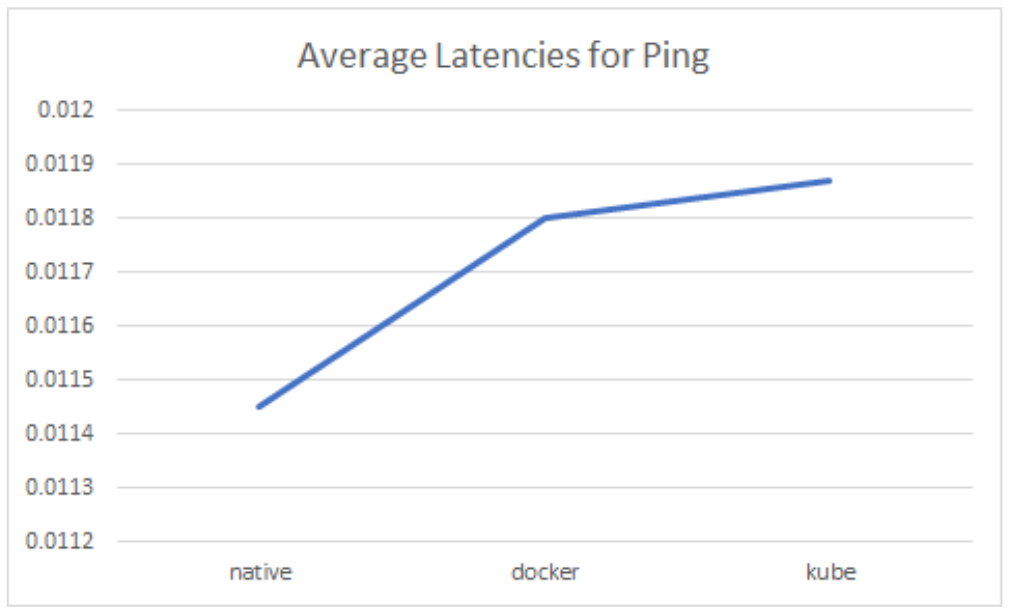
\includegraphics[width=.8\linewidth]{figures/ping.png} 
    \caption{Ping Tasks} 
    \vspace{4ex}
  \end{minipage}%%
  \begin{minipage}[b]{0.33\linewidth}
    \centering
    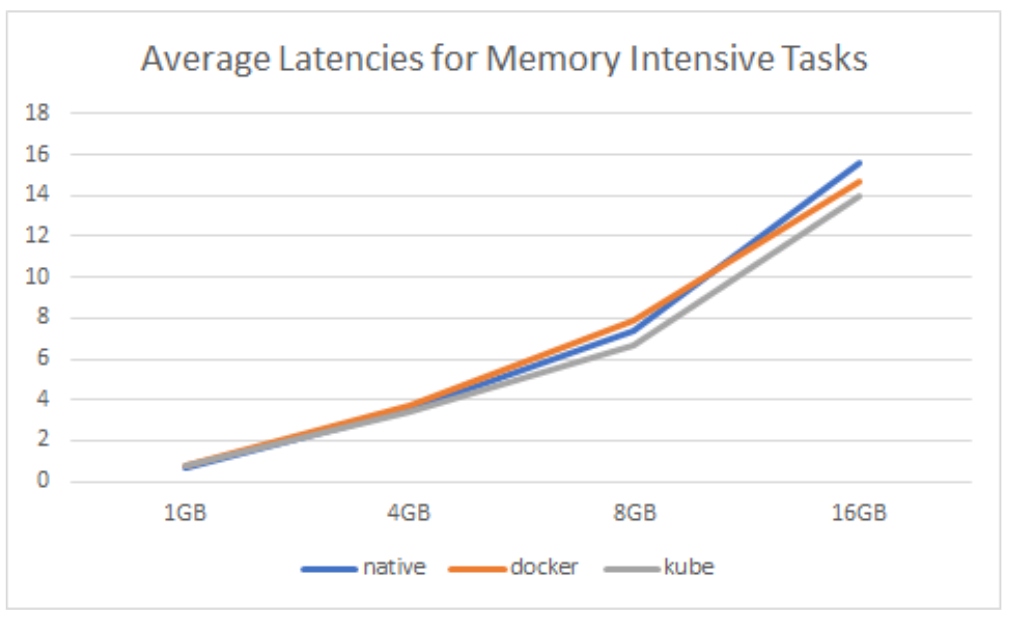
\includegraphics[width=.8\linewidth]{figures/mem.png} 
    \caption{Memory Intensive Tasks} 
    \vspace{4ex}
  \end{minipage}%%
  \begin{minipage}[b]{0.33\linewidth}
    \centering
    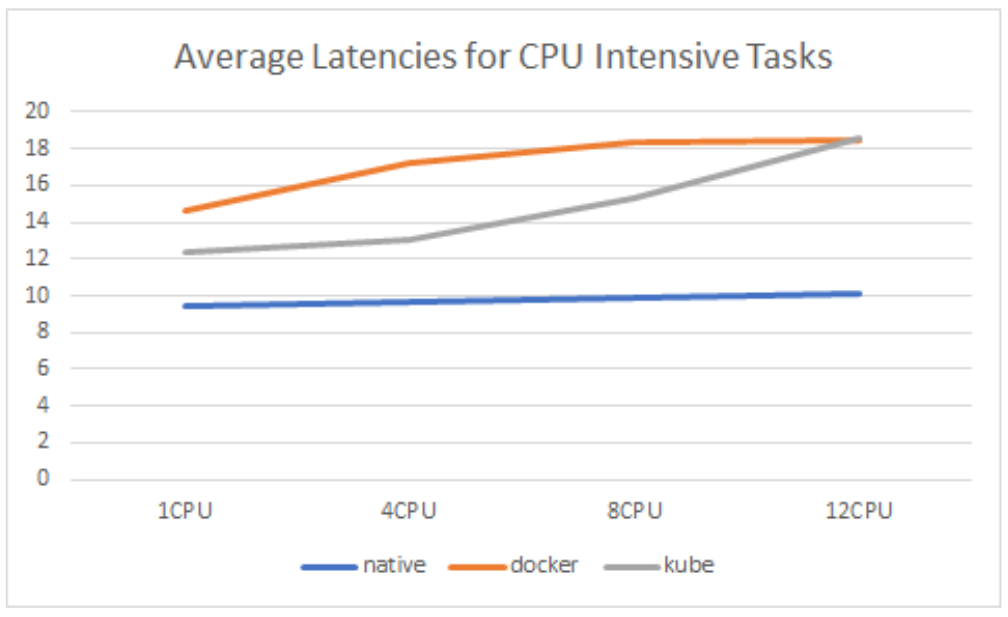
\includegraphics[width=.8\linewidth]{figures/CPU.png} 
    \caption{CPU Intensive Tasks} 
    \vspace{4ex}
  \end{minipage}
\end{figure*}

\section{Experiments}
We designed and conducted a set of basic experiments to evaluate the performance of Kubernetes cluster. The application containing these tests was deployed in 3 different environments - a Kubernetes cluster, a Docker container, and bare metal. For each test, we ran the experiment 100 times and recorded the latency values for the average, 10th percentile and 90th percentile case. The experiments are outlined as follows:

\subsection{Ping Test}
In the ping test, a simple "ping" request is sent to the application. The application responds with a simple acknowledgement. This test helps us get an idea of the overall overhead introduced by Kubernetes in the request response path.

\subsection{Memory Intensive Test}
We send a request to the application to perform a memory-intensive task. The request specifies an amount of memory to be allocated and also defines the time interval \texttt{t} for which to define it. The application creates and fills a data structure to occupy the specified size of memory, sleeps for \texttt{t} seconds, and then frees the memory. For our tests, we recorded latencies for requests with memory values of 1GB, 4GB, 8GB, and 16GB. Each size of memory is allocated for \texttt{t=0} seconds, which means the memory is freed right at the end of the time needed to allocate it. 

\subsection{CPU Intensive Test}
For the CPU intensive workload, we compute large exponents of a number. We also specify the number of CPUs we wish to run our computation on. For \texttt{n} number of CPUs, the computation is done \texttt{n} times parallely. We record latencies for requests with 1, 4, 8, and 12 CPUs.

\subsection{Results}
We observe latency overhead in the Kubernetes deployment of the application as opposed to bare metal. This overhead can be attributed to the runtime performance cost of Docker containers, caused due to port mapping between the host and the container. The results are outlined in Figures 2, 3 and 4.

\begin{table*}[]
    \centering
    \begin{tabular}{|c|c|c|}
        \hline
        \textbf{Cluster Domain} & \textbf{Service} & \textbf{StatefulSet} \\
        \hline
        cluster.local & default/ngnix & default/web \\
        \hline
        \textbf{StatefulSet Domain} & \textbf{Pod DNS} & \textbf{Pod Hostname} \\
        \hline
        nginx.default.svc.cluster.local & web-\{0..N-1\}.nginx.default.svc.cluster.local & web-\{0..N-1\} \\ 
        \hline
    \end{tabular}
    \caption{Example Network ID}
    \label{tab:Stateful Network}
\end{table*}

\section{Case Study - Running MongoDB on Kubernetes}
MongoDB is a powerful cross-platform NoSQL database application. It is widely used by applications that require flexible data model, scalability and strong performance. Ever since the birth of Kubernetes, there has been a line of work on deploying and running MongoDB with Kubernetes done by the open source community. This section will first look into the motivation and challenges of running MongoDB on Kubernetes. It will then cover a detailed deployment process as well as a performance comparison with various workload between native MongoDB cluster and Kubernetes MongoDB cluster.

\subsection{What Kubernetes can offer}
As one of the most widely used orchestration frameworks, Kubernetes combines the advantages of containers and container scheduling system \cite{mongoDBWhitePaper}. Below are some benefits of using containerized applications.
\begin{itemize}
    \item \textbf{Isolation}. In Kubernetes, each container runs an application in a completely isolated environment from other containers so that developers do not need to worry about the conflict of configuration between applications. Such isolation also improves the stability of the cluster since the crash of one application cannot affect applications running in a separate container.
    \item \textbf{Automated Deployment}. Kubernetes supports elastic scaling of container instances. In case developers want to add/remove containers or do an upgrade on the application, Kubernetes can perform scaling and rolling upgrade automatically without taking down the whole cluster.
    \item \textbf{Automated Rescheduling of Failed Containers}. As described in Section 5, the powerful failure recovery mechanism is arguably the most important motivation of running MongoDB on Kubernetes. Consider a native MongoDB cluster with replication set of 3 nodes, in case of node failure, the database administrator has to manually create a new MongoDB instance, configure it with the same setup as other node in the replication set and join it back to the cluster which could be quite a complicated process. However, by using Kubernetes, such node failures can be handled automatically without any admin interference.
\end{itemize}

\subsection{Challenges}
Running MongoDB on Kubernetes is not trivial \cite{mongoDBMicroservice}. This section looks into some of the addition considerations introduced by Kubernetes.
\begin{itemize}
    \item \textbf{Stateful Application}. MongoDB database itself is a stateful application which means a node needs to remember its previous state especially for the data after coming back from failure. However, in contrast, containers are mortal. Everything including storage will disappear when a container goes down. In order to solve this, a persistent volume needs to be attached to MongoDB application containers.  
    \item \textbf{Network Communication}. Nodes within the same MongoDB replication set need to communicate with each other in order to perform back up and synchronization. This implies that every node needs to know each other's network address. However, in a normal Kubernetes service, a pod will be assigned a different ID as well as IP address after coming back from failure which is problematic for communication within the replication set.
    \item \textbf{MongoDB Initialization}. After setting up an individual MongoDB instance, developers still need to initialize the MongoDB replication set by executing command inside mongo shell on one the instances. This indicates that developers need to find a way to directly talk to the application running inside the container.
\end{itemize}


\subsection{Kubernetes StatefulSet}
In order to address the challenges mentioned above, Kubernetes introduces a new concept called StatefulSet\cite{StatefulSets} which is a workload API object used to manage stateful applications. StatefulSet guarantees a stable and unique network together with a stable and persistent storage for the pods running in the cluster.

\subsubsection{Stable Network ID}
Once a pod is created, it will be assigned with a unique integer ordinal within the StatefulSet. The pod then derives its hostname by following the pattern \emph{ \$(statefulset name)-\$(ordinal)}. A StatefulSet also has a Headless Service that controls the domain of its pod. The domain of this service is given in the form of\emph{ \$(service name).\$(namespace).svc.cluster.local}. And each Pod will be assigned a DNS of the form of \emph{\$(pod name).\$(service domain)}. Table 1 shows an example Stable Network ID for a Kubernetes StatefulSet. 

\subsubsection{Stable Storage}
Kubernetes creates one persistent volume for each persistent volume claim. The pod will always be mounted on the persistent volume associated with its persistent volume claim even after coming back from crash. Details about creating persistent volume in Kubernetes will be addressed in the next section.

\subsubsection{Limitations} 
The current implementation of Kubernetes StatefulSet still has the following limitations.
\begin{itemize}
    \item \textbf{Storage Creation} Currently, there are two ways to create persistent storage for a StatefulSet. One is to provision storage through Persistent Volume Provisioner which means in order to enable dynamic storage allocation, developers have to configure the cluster with the Provisioner's service first. The other way is to pre-provision enough static persistent volume and allocate to the MongoDB application running in a StatefulSet which does not scale well. Both methods require enormous time and effort for the administrator to configure.
    \item \textbf{Storage Recollection} Removing a StatefulSet does not delete its associated persistent storage. Kubernetes claims that this is desirable since data safety is more important than resource recollection. However, in the case that developers do not want the associated storage, deletion has to be done manually.
    \item \textbf{StatefulSet Deletion} Deleting a StatefulSet does not guarantee the termination of all pods within the StatefulSet. The solution suggested by Kubernetes is to first scale down the StatefulSet to size 0 and then delete. This will make sure that all pods are terminated prior to deletion.
\end{itemize}

\begin{figure*}[ht] 
  \label{mongo} 
  \begin{minipage}[b]{0.45\linewidth}
    \centering
    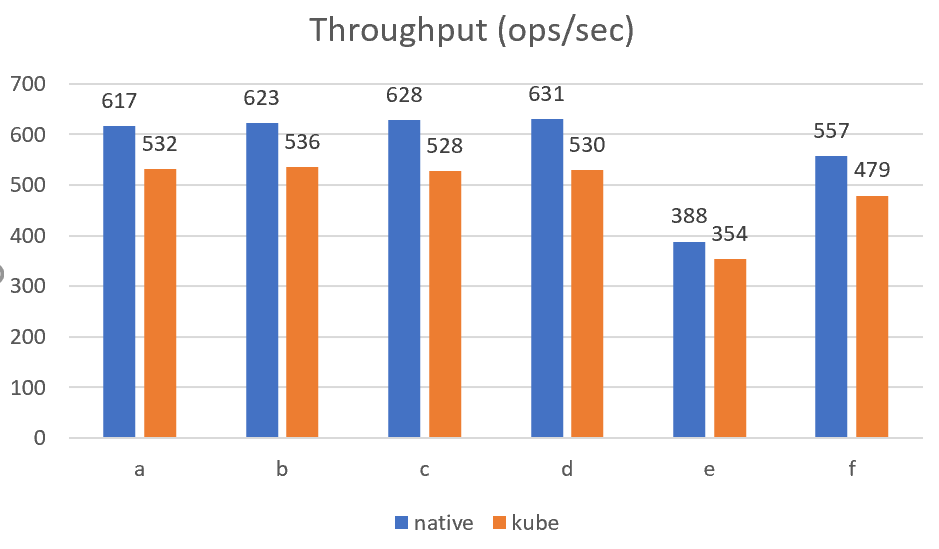
\includegraphics[width=.8\linewidth]{figures/throughput.png} 
    \caption{Throughput} 
    \vspace{4ex}
  \end{minipage}%%
  \begin{minipage}[b]{0.45\linewidth}
    \centering
    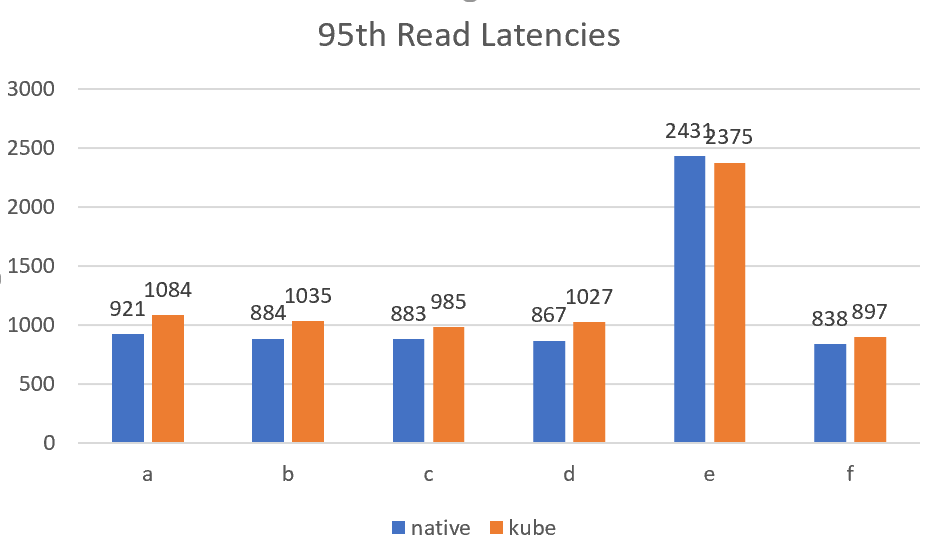
\includegraphics[width=.8\linewidth]{figures/95th.png} 
    \caption{95 Percentile Read Latency} 
    \vspace{4ex}
  \end{minipage} 
  \begin{minipage}[b]{0.45\linewidth}
    \centering
    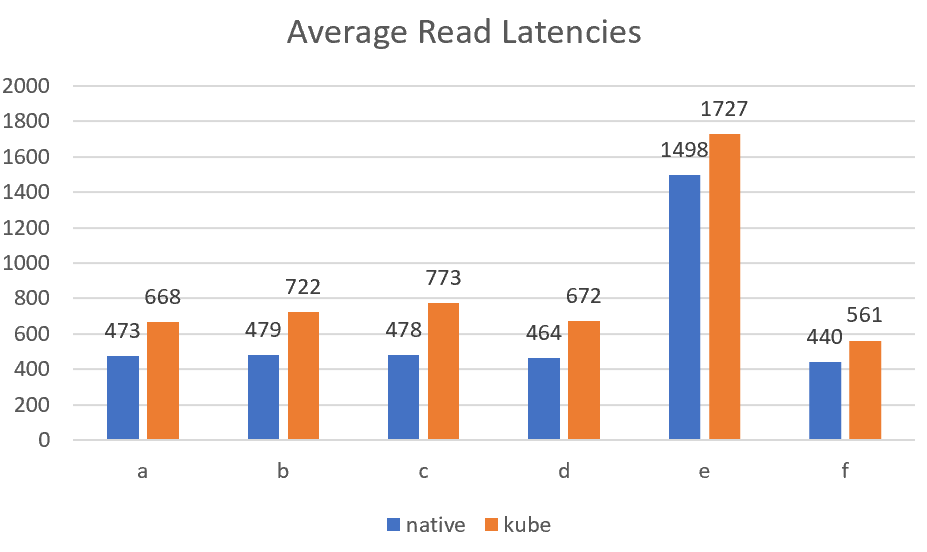
\includegraphics[width=.8\linewidth]{figures/average.png} 
    \caption{Average Read Latency} 
    \vspace{4ex}
  \end{minipage}%% 
  \begin{minipage}[b]{0.45\linewidth}
    \centering
    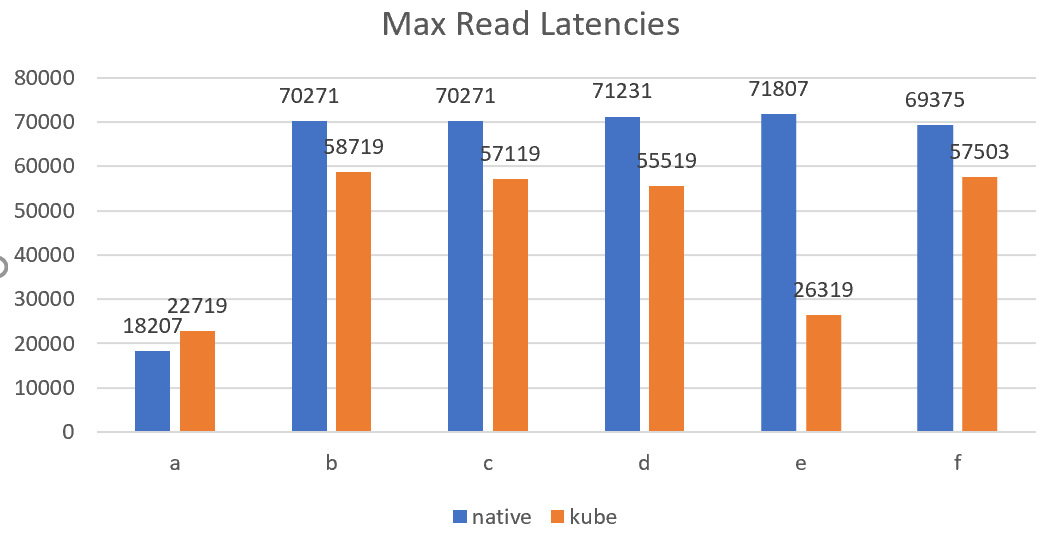
\includegraphics[width=.8\linewidth]{figures/max.png} 
    \caption{Maximum Read Latency} 
    \vspace{4ex}
  \end{minipage} 
\end{figure*}

\subsection{Deployment Setup}
We utilize 4 nodes named yellow 12-15 on the University of Waterloo SYN cluster, each of which runs Ubuntu 16.04. All the nodes share 64GB of memory, a 12 core CPU and similar network stack so that they can communicate with each other freely. Two MongoDB replication sets are deployed on yellow 13-15. Yellow 12 is used as the testing server so no application runs on it.

We first deploy a native MongoDB replication set using 3 nodes with yellow 14 as the primary set. All configurations are set to default. User can use MongoDB service by accessing the address \emph{yellow14:27017}. Note that MongoDB does not allow direct writing on secondary replicas so exposing primary replication address is sufficient.

We then deploy an identical MongoDB replication set with Kubernetes. Yellow 13 is used as the Kubernetes master and yellow 14 is chosen as the primary replication which exposes its service as type NodePort. For the Kubernetes deployment, we use the StatefulSet approach with dynamic storage allocation as described in the previous section. User can use MongoDB service by accessing \emph{yellow13:\$(exposed service port)}.

\subsection{Failover Test}
A failover test is conducted on Kubernetes MongoDB replication set in order to understand how Kubernetes handles pod failure in a MongoDB replication set.

The initial state is that 3 pods, each of which have a MongoDB instance, named db-0, db-1 and db-2 are running in the cluster with db-0 being the primary replication. When we take down the pod db-0, MongoDB notices that the primary replication goes down and elects db-1 as the new primary replication. Meanwhile, Kubernetes notices that one of the pods goes down so it will start the failover mechanism by creating a new pod and joining it back to the cluster as a secondary replication. The new pod will have the same network identity within the StatefulSet. In the final state after failure recovery, there are 3 pods with the same name db-0, db-1 and db-2, and db-1 serves as the primary replication. 

\subsection{Benchmark}
Apart from failover test, we also run various workloads on the two clusters. This section will first introduce the workload followed by an evaluation of the performance of two clusters.

\subsubsection{YCSB workload}
The Yahoo! Cloud Serving Benchmark (YCSB) \cite{ycsb} is a widely used benchmarking tool to measure database application performance. We test 6 different workloads as described in the following.
\begin{itemize}
    \item \textbf{Workload A: Update heavy workload}. 50\% of read and 50\% of write. Application example: session store recording recent actions.
    \item \textbf{Workload B: Read mostly workload}. 95\% of read and 5\% of write. Application example: photo tagging.
    \item \textbf{Workload C: Read only workload}. 100\% of read. Application example: user profile cache.
    \item \textbf{Workload D: Read latest workload}. Newly inserted records are more likely to be read. Application example: user status update.
    \item \textbf{Workload E: Short ranges}. Perform range queries only. Application example: geographic location scan.
    \item \textbf{Workload F: Read-modify-write}. Read a record, modify it and write back to the database. Application example: record update.
\end{itemize}

\subsubsection{Results}
Figures 6 and 7 show the 95 percentile read latency and average read latency on two clusters. Since the maximum latency is pretty high in our test, it may be a better reflection of cluster performance. We observe that Kubernetes in general has a higher read latency in most of the cases. The only exception is the range query workload (workload e) where linear scan become the dominating time. The results also match our previous result in the ping experiment where Kubernetes introduce certain amount of communication overhead compared to native clusters. Due to the communication overhead, the throughput in terms of operations per second for Kubernetes cluster is also smaller than native cluster as shown in Figure 5. It seems that developers are sacrificing a small part of performance in exchange for the powerful features provided by Kubernetes.

We also observe a result that is beyond our expectation where Kubernetes has a lower tail latency compared with native cluster as shown in Figure 8. We think this result may be due to our experiment setup. Since the native MongoDB cluster is running on 3 different nodes, when the primary replication wants to direct the read to a secondary replication, it has to jump between machines. While in Kubernetes cluster, although it also runs on 3 different nodes, the master node is configured as a non-work node to achieve better isolation. Therefore, 2 pods actually run on the same machine and have less communication overhead. As a result, tail latency is smaller in Kubernetes cluster.

\section{Conclusion}
We study Kubernetes as a container orchestration layer and dissect its features that enable it to provide high availability and easy deployment of distributed containerized applications. Through our experiments and benchmarks, we conclude that while Kubernetes has a performance impact on the application, it provides the tools needed to deploy quickly while staying available. These ideas improve the overall velocity of reliable software deployment.


%%
%% The next two lines define the bibliography style to be used, and
%% the bibliography file.
\bibliographystyle{ACM-Reference-Format}
\bibliography{sample-base}

%%
%% If your work has an appendix, this is the place to put it.
\appendix

\section{Kubernetes Practice}
This section introduces some of the difficulties we encountered when installing, deploying and running kubernetes. A detailed work pipeline has been uploaded to our github repo \footnote{\url{https://github.com/udhavsethi/kube-play}}. This workflow works perfectly on SYN cluster and should also work on other clusters as well.

\subsection{Firewall issues}
Here we struggled with making sure all nodes in your Kubernetes cluster can communicate with each other. Previously we were running Kubernetes on machines within different networks, such setup is not recommended since the firewall may block the incoming Kubernetes connections and leads to unexpected behavior. Using cluster is strongly recommended.

\subsection{Change of IP address}
Once a Kubernetes cluster is set up, nodes can be added or removed easily from the cluster. However, changing master node IP and restart cluster is not recommended. The previous IP address is written in Kubernetes configuration file and cannot be reset through Kubeadm. Changing master IP may cause work nodes unable to join the cluster.

\subsection{Working with NFS}
Many clusters leverage NFS techniques to mount single user's nodes to the same mount point. So all these nodes will share the same storage and files. Such design is quite convenient in most of the cases. However, when using with Kubernetes, the same configuration file is distributed across all the machines. We haven't found a practical solution to deploy two different Kubernetes on the cluster since one configuration file will overwrite the other's file.

\section{MongoDB PRACTICE}
This section discusses some of the difficulties we encountered when deploying native MongoDB cluster and Kubernetes MongoDB cluster.

\subsection{MongoDB replication set}
Make sure your nodes can talk with each other before setting up replication set. To initiate a replication set, developers need to go into one of the MongoDB instances to execute some mongo shell command. The set up is in general not trivial. 

Apart from the set up, MongoDB has some weird configurations that I do not quite understand. For example, if localhost is used in the configuration of replication set, then either all the replicas are configured with localhost or none of then should be configured with localhost. Also, once the replication set is initiated, there is no elegant way to destroy it.

\subsection{MongoDB on Kubernetes}
We spend so much time trying to deploy MongoDB on Kubernetes that you can not imagine. We start by trying Kubernetes MongoDB operators which provides a fancy cloud controller with web interface but their documentation doesn't really work.

Later on we switch to Kubernetes StatefulSet which is easier to get it work but still it takes a lot of time and effort. To enable dynamic storage allocation, one needs to configure the cluster with a Persistent Volume Provisioner. I would recommend to simply use static storage allocation which is arguably the easiest approach to get an persistent storage in your cluster. 

\end{document}
\endinput
%%
%% End of file `sample-sigconf.tex'.
